\section{Information loss}\label{sec:info}

Windows also destroy transition information, which we measure by the compression term of the Brier score. Let $Z$ be the latent Markov state, $E\in\{0,1\}$ an event, $\pOp(Z)=\mathrm P(E=1\mid Z)$ the oracle, $Y$ the observed state and $r^*(Y)=\mathrm P(E=1\mid Y)$. For any forecast $g(Y)$, orthogonality of the three differences gives the standard decomposition \cite{murphy1973,degroot1983,brocker2009}
\begin{align}
\E[(g-E)^2]&=\E[(g-r^*)^2]+\E[(r^*-\pOp)^2]\nonumber\\
&\quad+\E[\pOp(1-\pOp)]
\end{align}
into an estimation, a compression and a state-information term. The compression term, $L=\E[\mathrm{Var}(\pOp\mid Y)]$, is what the observer loses by seeing $Y$ instead of $Z$, whatever estimator it uses; we report it normalized, $\ell=L/\mathrm{Var}\,\pOp\in[0,1]$.

\subsection{Gaussian observer: an exact series}\label{sec:mehler}

For a reversible Ornstein--Uhlenbeck input the compression term is an exact Hermite series in the posterior variance. Given the windows $y_t$, the latent state is Gaussian with a mean linear in $y_t$ and a variance $s^2=1-c^\top C(0)^{-1}c$, $c_i=\mathrm{Cov}(x_t,y_i(t))$, that does not depend on the observed values.

\begin{lemma}[Mehler series]\label{lem:mehler}
If $\pOp$ has the normalized Hermite coefficients $a_n=\E[\pOp(X)\,\mathrm{He}_n(X)]/\sqrt{n!}$ under $X\sim N(0,1)$, then
\begin{equation}
L(s^2)=\sum_{n\ge1}a_n^2\big[1-(1-s^2)^n\big].\label{eq:mehler}
\end{equation}
$L$ increases from $L(0)=0$ to $L(1)=\mathrm{Var}\,\pOp$, and $L'(0)=\E[\pOp'(X)^2]\ge\mathrm{Var}\,\pOp$.
\end{lemma}

This is the classical Hermite (Mehler) expansion of the Ornstein--Uhlenbeck semigroup \cite{mehler1866,odonnell2014}, applied to the posterior of the latent state (Appendix~\ref{app:gauss}); the last inequality is the Gaussian Poincar\'e inequality and says that threshold events lose information faster than linear ones. Figure~\ref{fig:gauss}(a) shows $\ell$ for windows $(w,4w)$, a threshold at $2\sigma$ and a horizon of ten steps, as in Table~\ref{tab:gauss}: the series agrees with the Monte Carlo loss of the exact Bayes observer on $3\times10^5$-step paths, and the curves for four values of $\phi$ approach one function of $\lambda w$ as the sampling becomes fine. The residual spread reflects discreteness of short windows at $\phi=0.9$, and at $\phi=0.99$ the simulated loss falls below the series by up to \MCDevNineNine of $\mathrm{Var}\,\pOp$ because a path then holds only about $10^3$ independent samples (Table~\Sref{gauss}).

\begin{figure*}[t]
\centering
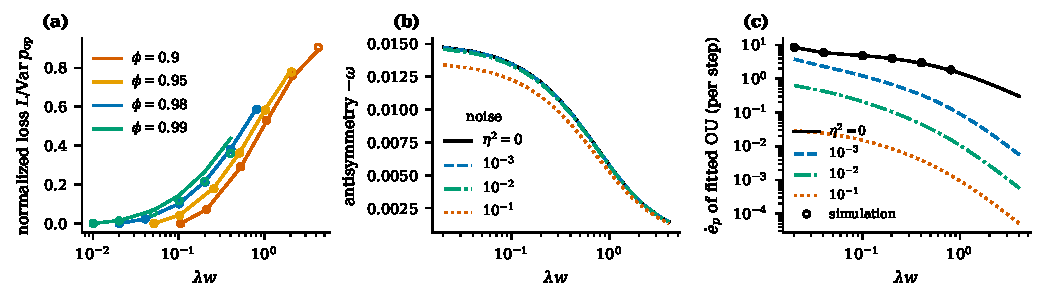
\includegraphics[width=\textwidth]{figures/fig2_gaussian_observer.pdf}
\caption{A reversible Ornstein--Uhlenbeck input seen through trailing windows $(w,4w)$ loses transition information and acquires a large fitted dissipation that is fixed by innovation geometry, not by the current. (a) Normalized compression loss of a threshold forecast (threshold $2\sigma$, horizon 10): lines, Eq.~\eqref{eq:mehler}; circles, Monte Carlo loss of the exact Bayes observer. (b) Lag-one antisymmetry for independent observation noise $\eta^2$ (relative to the window variance); it changes only through the noise-inflated variances. (c) Entropy production of the fitted OU model for the same noise levels; circles, simulation without noise.}
\label{fig:gauss}
\end{figure*}

\subsection{Double well: two rates}\label{sec:dw}

In a double well the compression term is governed by two rates: the local curvature within wells and the Kramers rate between them. The test system is $dx=-(x^3-x-c_t)\,dt+0.72\,dW^{(x)}$, $dc=-c\,\tau_c^{-1}dt+0.18\,dW^{(c)}$ with $\tau_c\in\{5,20,80,\infty\}$ ($c\equiv0$ for $\tau_c=\infty$), integrated with Euler steps of $0.05$; the event is $x\ge0.65$ within two time units, scored from states with $x<0.65$, and the oracle $\pOp(x,c)$ follows from the known generator. This is the textbook model of bifurcation- and noise-induced tipping \cite{ashwin2012}. The observer sees trailing means of $x$ and $c$ over $w$ steps. We estimate $L$ directly as the out-of-sample mean squared residual of a flexible regression of $\pOp$ on the observation, trained on $7\times10^5$ steps; at $w=1$ the estimate is below $10^{-3}$ (Appendix~\ref{app:tworate}).

A single-rate Gaussian theory with the local stiffness $\bar\lambda=\E[U''(x_L)]\simeq2$ predicts $\ell=s^2(\bar\lambda w)$ and overestimates the loss by between \SingleErrLo and \SingleErrHi [Fig.~\ref{fig:dw}(b)]. The reason is visible in the autocorrelation of $x$ [Fig.~\ref{fig:dw}(a)]: it decays with two rates, and the slow one ($0.169$) is the Kramers switching rate $\kappa=k_{L\to R}+k_{R\to L}=0.172$ \cite{kramers1940,hanggi1990}, not the curvature. The oracle inherits this structure: 85\% of $\mathrm{Var}\,\pOp$ lies between the two sides of the barrier and only 15\% within them, and a trailing window resolves the side for times shorter than $1/\kappa$. Splitting $\mathrm{Var}\,\pOp=V_b+V_w$ by the side and weighting each part by the posterior variance of its own rate gives the two-rate approximation
\begin{equation}
\ell(w)\simeq\frac{V_b\,s^2(\kappa w)+V_w\,s^2(\bar\lambda w)}{\mathrm{Var}\,\pOp},\label{eq:tworate}
\end{equation}
evaluated conditionally on $c$ for finite $\tau_c$, with Kramers rates of the tilted well and no fitted parameter. It reduces the error from between \SingleErrLo and \SingleErrHi to between \TwoErrLo and \TwoErrHi (Table~\Sref{dwloss}): the mechanism is right, and the remaining underestimate at the widest windows comes from hops inside the window, where the posterior of the side is far from Gaussian. The exact losses for the four control time scales nearly coincide at fixed $\bar\lambda w$. Estimating the same loss from the skill difference of a classifier trained on $8.4\times10^3$ points overstates it (\ClfEst against \ClfExact at $\tau_c=5$, $w=80$; Table~\Sref{dwloss}), because the classifier on wide windows loses skill to estimation rather than to compression.

\begin{figure*}[t]
\centering
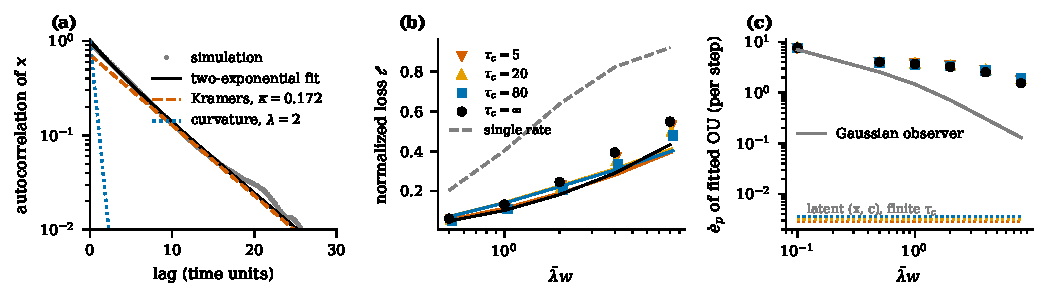
\includegraphics[width=\textwidth]{figures/fig3_double_well.pdf}
\caption{In the double well the loss is governed by two rates, and a two-window observer of a reversible well reports a large current. (a) Autocorrelation of $x$ for $\tau_c=\infty$: a fast intra-well part and a slow part decaying at the Kramers rate $\kappa$ (dashed), far from the curvature rate (dotted). (b) Normalized compression loss: markers, near-exact Bayes loss for four $\tau_c$; lines, two-rate approximation~\eqref{eq:tworate}; dashed, single-rate Gaussian theory. (c) Entropy production of the OU model fitted to two trailing windows $(w,4w)$ of $x$ alone (markers); dotted, the latent $(x,c)$ value for finite $\tau_c$; line, Gaussian observer with $\bar\lambda$ (Sec.~\ref{sec:gauss}).}
\label{fig:dw}
\end{figure*}
